\documentclass[12pt,a4paper]{article}

\usepackage[a4paper,text={16.5cm,25.2cm},centering]{geometry}
\usepackage{lmodern}
\usepackage{amssymb,amsmath}
\usepackage{bm}
\usepackage{graphicx}
\usepackage{microtype}
\usepackage{hyperref}
\setlength{\parindent}{0pt}
\setlength{\parskip}{1.2ex}

\hypersetup
       {   pdfauthor = { Viktor Bílek },
           pdftitle={ The Effect of the Loss Function on Quality of Anomaly Detection },
           colorlinks=TRUE,
           linkcolor=black,
           citecolor=blue,
           urlcolor=blue
       }

\title{ The Effect of the Loss Function on Quality of Anomaly Detection }

\author{ Viktor Bílek }

\date{ 12.11.2020 }

\usepackage{upquote}
\usepackage{listings}
\usepackage{xcolor}
\lstset{
    basicstyle=\ttfamily\footnotesize,
    upquote=true,
    breaklines=true,
    breakindent=0pt,
    keepspaces=true,
    showspaces=false,
    columns=fullflexible,
    showtabs=false,
    showstringspaces=false,
    escapeinside={(*@}{@*)},
    extendedchars=true,
}
\newcommand{\HLJLt}[1]{#1}
\newcommand{\HLJLw}[1]{#1}
\newcommand{\HLJLe}[1]{#1}
\newcommand{\HLJLeB}[1]{#1}
\newcommand{\HLJLo}[1]{#1}
\newcommand{\HLJLk}[1]{\textcolor[RGB]{148,91,176}{\textbf{#1}}}
\newcommand{\HLJLkc}[1]{\textcolor[RGB]{59,151,46}{\textit{#1}}}
\newcommand{\HLJLkd}[1]{\textcolor[RGB]{214,102,97}{\textit{#1}}}
\newcommand{\HLJLkn}[1]{\textcolor[RGB]{148,91,176}{\textbf{#1}}}
\newcommand{\HLJLkp}[1]{\textcolor[RGB]{148,91,176}{\textbf{#1}}}
\newcommand{\HLJLkr}[1]{\textcolor[RGB]{148,91,176}{\textbf{#1}}}
\newcommand{\HLJLkt}[1]{\textcolor[RGB]{148,91,176}{\textbf{#1}}}
\newcommand{\HLJLn}[1]{#1}
\newcommand{\HLJLna}[1]{#1}
\newcommand{\HLJLnb}[1]{#1}
\newcommand{\HLJLnbp}[1]{#1}
\newcommand{\HLJLnc}[1]{#1}
\newcommand{\HLJLncB}[1]{#1}
\newcommand{\HLJLnd}[1]{\textcolor[RGB]{214,102,97}{#1}}
\newcommand{\HLJLne}[1]{#1}
\newcommand{\HLJLneB}[1]{#1}
\newcommand{\HLJLnf}[1]{\textcolor[RGB]{66,102,213}{#1}}
\newcommand{\HLJLnfm}[1]{\textcolor[RGB]{66,102,213}{#1}}
\newcommand{\HLJLnp}[1]{#1}
\newcommand{\HLJLnl}[1]{#1}
\newcommand{\HLJLnn}[1]{#1}
\newcommand{\HLJLno}[1]{#1}
\newcommand{\HLJLnt}[1]{#1}
\newcommand{\HLJLnv}[1]{#1}
\newcommand{\HLJLnvc}[1]{#1}
\newcommand{\HLJLnvg}[1]{#1}
\newcommand{\HLJLnvi}[1]{#1}
\newcommand{\HLJLnvm}[1]{#1}
\newcommand{\HLJLl}[1]{#1}
\newcommand{\HLJLld}[1]{\textcolor[RGB]{148,91,176}{\textit{#1}}}
\newcommand{\HLJLs}[1]{\textcolor[RGB]{201,61,57}{#1}}
\newcommand{\HLJLsa}[1]{\textcolor[RGB]{201,61,57}{#1}}
\newcommand{\HLJLsb}[1]{\textcolor[RGB]{201,61,57}{#1}}
\newcommand{\HLJLsc}[1]{\textcolor[RGB]{201,61,57}{#1}}
\newcommand{\HLJLsd}[1]{\textcolor[RGB]{201,61,57}{#1}}
\newcommand{\HLJLsdB}[1]{\textcolor[RGB]{201,61,57}{#1}}
\newcommand{\HLJLsdC}[1]{\textcolor[RGB]{201,61,57}{#1}}
\newcommand{\HLJLse}[1]{\textcolor[RGB]{59,151,46}{#1}}
\newcommand{\HLJLsh}[1]{\textcolor[RGB]{201,61,57}{#1}}
\newcommand{\HLJLsi}[1]{#1}
\newcommand{\HLJLso}[1]{\textcolor[RGB]{201,61,57}{#1}}
\newcommand{\HLJLsr}[1]{\textcolor[RGB]{201,61,57}{#1}}
\newcommand{\HLJLss}[1]{\textcolor[RGB]{201,61,57}{#1}}
\newcommand{\HLJLssB}[1]{\textcolor[RGB]{201,61,57}{#1}}
\newcommand{\HLJLnB}[1]{\textcolor[RGB]{59,151,46}{#1}}
\newcommand{\HLJLnbB}[1]{\textcolor[RGB]{59,151,46}{#1}}
\newcommand{\HLJLnfB}[1]{\textcolor[RGB]{59,151,46}{#1}}
\newcommand{\HLJLnh}[1]{\textcolor[RGB]{59,151,46}{#1}}
\newcommand{\HLJLni}[1]{\textcolor[RGB]{59,151,46}{#1}}
\newcommand{\HLJLnil}[1]{\textcolor[RGB]{59,151,46}{#1}}
\newcommand{\HLJLnoB}[1]{\textcolor[RGB]{59,151,46}{#1}}
\newcommand{\HLJLoB}[1]{\textcolor[RGB]{102,102,102}{\textbf{#1}}}
\newcommand{\HLJLow}[1]{\textcolor[RGB]{102,102,102}{\textbf{#1}}}
\newcommand{\HLJLp}[1]{#1}
\newcommand{\HLJLc}[1]{\textcolor[RGB]{153,153,119}{\textit{#1}}}
\newcommand{\HLJLch}[1]{\textcolor[RGB]{153,153,119}{\textit{#1}}}
\newcommand{\HLJLcm}[1]{\textcolor[RGB]{153,153,119}{\textit{#1}}}
\newcommand{\HLJLcp}[1]{\textcolor[RGB]{153,153,119}{\textit{#1}}}
\newcommand{\HLJLcpB}[1]{\textcolor[RGB]{153,153,119}{\textit{#1}}}
\newcommand{\HLJLcs}[1]{\textcolor[RGB]{153,153,119}{\textit{#1}}}
\newcommand{\HLJLcsB}[1]{\textcolor[RGB]{153,153,119}{\textit{#1}}}
\newcommand{\HLJLg}[1]{#1}
\newcommand{\HLJLgd}[1]{#1}
\newcommand{\HLJLge}[1]{#1}
\newcommand{\HLJLgeB}[1]{#1}
\newcommand{\HLJLgh}[1]{#1}
\newcommand{\HLJLgi}[1]{#1}
\newcommand{\HLJLgo}[1]{#1}
\newcommand{\HLJLgp}[1]{#1}
\newcommand{\HLJLgs}[1]{#1}
\newcommand{\HLJLgsB}[1]{#1}
\newcommand{\HLJLgt}[1]{#1}


\begin{document}

\maketitle

\section{Introduction}
Comparison of maximum-likelihood and quantile likelihood loss function for anomaly detection using SPTN model.

%  this setup dependencies, but doesn't appear in the generated document 


\section{Definition of SPTN model}

\begin{lstlisting}
(*@\HLJLk{function}@*) (*@\HLJLnf{sptn}@*)(*@\HLJLp{(}@*)(*@\HLJLn{d}@*)(*@\HLJLp{,}@*) (*@\HLJLn{n}@*)(*@\HLJLp{,}@*) (*@\HLJLn{l}@*)(*@\HLJLp{)}@*)
	(*@\HLJLn{m}@*) (*@\HLJLoB{=}@*) (*@\HLJLnf{TransformationNode}@*)(*@\HLJLp{(}@*)(*@\HLJLnf{ScaleShift}@*)(*@\HLJLp{(}@*)(*@\HLJLn{d}@*)(*@\HLJLp{),}@*)  (*@\HLJLnf{TuringMvNormal}@*)(*@\HLJLp{(}@*)(*@\HLJLn{d}@*)(*@\HLJLp{,}@*)(*@\HLJLnfB{1f0}@*)(*@\HLJLp{))}@*)
	(*@\HLJLk{for}@*) (*@\HLJLn{i}@*) (*@\HLJLkp{in}@*) (*@\HLJLni{1}@*)(*@\HLJLoB{:}@*)(*@\HLJLn{l}@*)
		(*@\HLJLn{m}@*) (*@\HLJLoB{=}@*) (*@\HLJLnf{SumNode}@*)(*@\HLJLp{([}@*)(*@\HLJLnf{TransformationNode}@*)(*@\HLJLp{(}@*)(*@\HLJLnf{SVDDense}@*)(*@\HLJLp{(}@*)(*@\HLJLni{2}@*)(*@\HLJLp{,}@*) (*@\HLJLn{identity}@*)(*@\HLJLp{,}@*) (*@\HLJLsc{:butterfly}@*)(*@\HLJLp{),}@*) (*@\HLJLn{m}@*)(*@\HLJLp{)}@*)
					(*@\HLJLk{for}@*) (*@\HLJLn{i}@*) (*@\HLJLkp{in}@*) (*@\HLJLni{1}@*)(*@\HLJLoB{:}@*)(*@\HLJLn{n}@*)(*@\HLJLp{])}@*)
	(*@\HLJLk{end}@*)
	(*@\HLJLk{return}@*)(*@\HLJLp{(}@*)(*@\HLJLn{m}@*)(*@\HLJLp{)}@*)
(*@\HLJLk{end}@*)
\end{lstlisting}

\begin{lstlisting}
sptn (generic function with 1 method)
\end{lstlisting}


\section{Anomaly detection with max-likelihood estimate loss}
Initialization of model and training data + anomalies. In this example we train model on data including anomalies.


\begin{lstlisting}
(*@\HLJLn{m}@*) (*@\HLJLoB{=}@*) (*@\HLJLnf{sptn}@*)(*@\HLJLp{(}@*)(*@\HLJLni{2}@*)(*@\HLJLp{,}@*) (*@\HLJLni{9}@*)(*@\HLJLp{,}@*) (*@\HLJLni{1}@*)(*@\HLJLp{)}@*)

(*@\HLJLn{x{\_}n}@*) (*@\HLJLoB{=}@*) (*@\HLJLnf{flower2}@*)(*@\HLJLp{(}@*)(*@\HLJLni{1000}@*)(*@\HLJLp{,}@*) (*@\HLJLn{npetals}@*)(*@\HLJLoB{=}@*)(*@\HLJLni{9}@*)(*@\HLJLp{)}@*)
(*@\HLJLn{x{\_}a}@*) (*@\HLJLoB{=}@*) (*@\HLJLnf{randn}@*)(*@\HLJLp{(}@*)(*@\HLJLni{2}@*)(*@\HLJLp{,}@*) (*@\HLJLni{10}@*)(*@\HLJLp{)}@*)
(*@\HLJLnf{scatter}@*)(*@\HLJLp{(}@*)(*@\HLJLn{x{\_}n}@*)(*@\HLJLp{[}@*)(*@\HLJLni{1}@*)(*@\HLJLp{,}@*) (*@\HLJLoB{:}@*)(*@\HLJLp{],}@*) (*@\HLJLn{x{\_}n}@*)(*@\HLJLp{[}@*)(*@\HLJLni{2}@*)(*@\HLJLp{,}@*) (*@\HLJLoB{:}@*)(*@\HLJLp{])}@*)
(*@\HLJLnf{scatter!}@*)(*@\HLJLp{(}@*)(*@\HLJLn{x{\_}a}@*)(*@\HLJLp{[}@*)(*@\HLJLni{1}@*)(*@\HLJLp{,}@*) (*@\HLJLoB{:}@*)(*@\HLJLp{],}@*) (*@\HLJLn{x{\_}a}@*)(*@\HLJLp{[}@*)(*@\HLJLni{2}@*)(*@\HLJLp{,}@*) (*@\HLJLoB{:}@*)(*@\HLJLp{])}@*)
(*@\HLJLn{x}@*) (*@\HLJLoB{=}@*) (*@\HLJLnf{shuffleobs}@*)(*@\HLJLp{(}@*)(*@\HLJLnf{hcat}@*)(*@\HLJLp{(}@*)(*@\HLJLn{x{\_}n}@*)(*@\HLJLp{,}@*) (*@\HLJLn{x{\_}a}@*)(*@\HLJLp{))}@*)
(*@\HLJLcs{{\#}scatter(x[1,}@*) (*@\HLJLcs{:],}@*) (*@\HLJLcs{x[2,}@*) (*@\HLJLcs{:])}@*)
(*@\HLJLn{{\_}data}@*) (*@\HLJLoB{=}@*) (*@\HLJLn{Iterators}@*)(*@\HLJLoB{.}@*)(*@\HLJLnf{repeated}@*)(*@\HLJLp{((),}@*) (*@\HLJLni{100}@*)(*@\HLJLp{)}@*)
\end{lstlisting}

\begin{lstlisting}
Base.Iterators.Take(*@{{\{}}@*)Base.Iterators.Repeated(*@{{\{}}@*)Tuple(*@{{\{}}@*)(*@{{\}}}@*)(*@{{\}}}@*)(*@{{\}}}@*)(Base.Iterators.Repeat
ed(*@{{\{}}@*)Tuple(*@{{\{}}@*)(*@{{\}}}@*)(*@{{\}}}@*)(()), 100)
\end{lstlisting}


Definition of loss function (max-likelihood) and start of training.


\begin{lstlisting}
(*@\HLJLnf{loss}@*)(*@\HLJLp{()}@*) (*@\HLJLoB{=}@*) (*@\HLJLoB{-}@*)(*@\HLJLnf{mean}@*)(*@\HLJLp{(}@*)(*@\HLJLnf{logpdf}@*)(*@\HLJLp{(}@*)(*@\HLJLn{m}@*)(*@\HLJLp{,}@*) (*@\HLJLn{x}@*)(*@\HLJLp{))}@*)

(*@\HLJLn{ps}@*) (*@\HLJLoB{=}@*) (*@\HLJLn{Flux}@*)(*@\HLJLoB{.}@*)(*@\HLJLnf{params}@*)(*@\HLJLp{(}@*)(*@\HLJLn{m}@*)(*@\HLJLp{)}@*)

(*@\HLJLn{opt}@*) (*@\HLJLoB{=}@*) (*@\HLJLnf{ADAM}@*)(*@\HLJLp{(}@*)(*@\HLJLnfB{0.1}@*)(*@\HLJLp{)}@*)
(*@\HLJLn{Flux}@*)(*@\HLJLoB{.}@*)(*@\HLJLn{Optimise}@*)(*@\HLJLoB{.}@*)(*@\HLJLnf{train!}@*)(*@\HLJLp{(()}@*) (*@\HLJLoB{->}@*) (*@\HLJLnf{loss}@*)(*@\HLJLp{(),}@*) (*@\HLJLn{ps}@*)(*@\HLJLp{,}@*) (*@\HLJLn{{\_}data}@*)(*@\HLJLp{,}@*) (*@\HLJLn{opt}@*)(*@\HLJLp{)}@*)
\end{lstlisting}


Heatmap of trained distribution.


\begin{lstlisting}
(*@\HLJLn{xx}@*) (*@\HLJLoB{=}@*) (*@\HLJLnf{reduce}@*)(*@\HLJLp{(}@*)(*@\HLJLn{hcat}@*)(*@\HLJLp{,[[}@*)(*@\HLJLn{v}@*)(*@\HLJLp{[}@*)(*@\HLJLni{1}@*)(*@\HLJLp{],}@*)(*@\HLJLn{v}@*)(*@\HLJLp{[}@*)(*@\HLJLni{2}@*)(*@\HLJLp{]]}@*) (*@\HLJLk{for}@*) (*@\HLJLn{v}@*) (*@\HLJLkp{in}@*) (*@\HLJLn{Iterators}@*)(*@\HLJLoB{.}@*)(*@\HLJLnf{product}@*)(*@\HLJLp{(}@*)(*@\HLJLoB{-}@*)(*@\HLJLnfB{10.0}@*)(*@\HLJLoB{:}@*)(*@\HLJLnfB{0.1}@*)(*@\HLJLoB{:}@*)(*@\HLJLni{10}@*)(*@\HLJLp{,}@*) (*@\HLJLoB{-}@*)(*@\HLJLnfB{10.0}@*)(*@\HLJLoB{:}@*)(*@\HLJLnfB{0.1}@*)(*@\HLJLoB{:}@*)(*@\HLJLni{10}@*)(*@\HLJLp{)])}@*)
(*@\HLJLn{res}@*) (*@\HLJLoB{=}@*) (*@\HLJLnf{reshape}@*)(*@\HLJLp{(}@*)(*@\HLJLnf{logpdf}@*)(*@\HLJLp{(}@*)(*@\HLJLn{m}@*)(*@\HLJLp{,}@*) (*@\HLJLn{xx}@*)(*@\HLJLp{),}@*) (*@\HLJLni{201}@*)(*@\HLJLp{,}@*) (*@\HLJLni{201}@*)(*@\HLJLp{)}@*)
(*@\HLJLn{Plots}@*)(*@\HLJLoB{.}@*)(*@\HLJLnf{heatmap}@*)(*@\HLJLp{(}@*)(*@\HLJLn{exp}@*)(*@\HLJLoB{.}@*)(*@\HLJLp{(}@*)(*@\HLJLn{res}@*)(*@\HLJLp{))}@*)
\end{lstlisting}

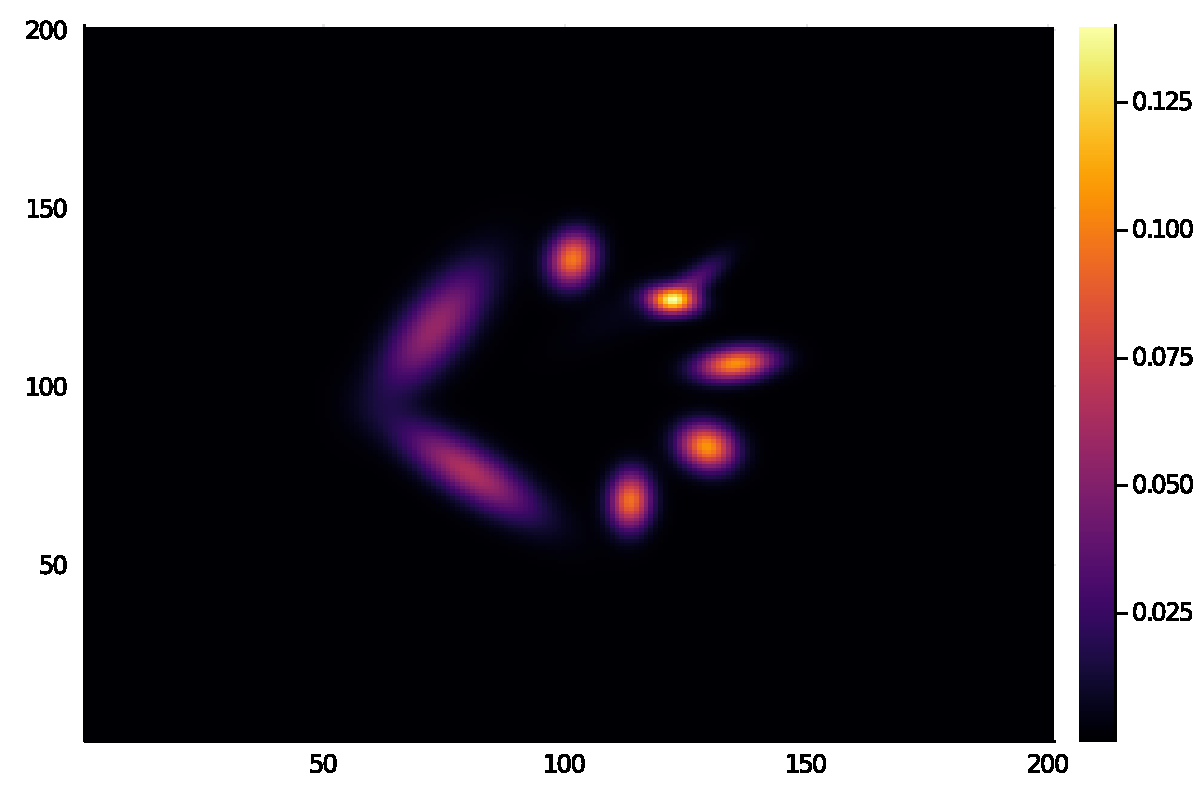
\includegraphics[width=\linewidth]{jl_uOl600/test1_5_1.pdf}

Scatter plot of anomaly detection.


\begin{lstlisting}
(*@\HLJLn{lkl}@*) (*@\HLJLoB{=}@*) (*@\HLJLnf{logpdf}@*)(*@\HLJLp{(}@*)(*@\HLJLn{m}@*)(*@\HLJLp{,}@*) (*@\HLJLn{x}@*)(*@\HLJLp{)}@*)
(*@\HLJLn{\ensuremath{\theta}}@*) (*@\HLJLoB{=}@*) (*@\HLJLnf{quantile{\_}tresh}@*)(*@\HLJLp{(}@*)(*@\HLJLn{lkl}@*)(*@\HLJLp{,}@*) (*@\HLJLnfB{0.01}@*)(*@\HLJLp{)}@*)

(*@\HLJLn{anom}@*)(*@\HLJLp{,}@*) (*@\HLJLn{norms}@*) (*@\HLJLoB{=}@*) (*@\HLJLnf{tresh{\_}lkl}@*)(*@\HLJLp{(}@*)(*@\HLJLn{m}@*)(*@\HLJLp{,}@*) (*@\HLJLn{x}@*)(*@\HLJLp{,}@*) (*@\HLJLn{\ensuremath{\theta}}@*)(*@\HLJLp{)}@*)
(*@\HLJLnf{scatter}@*)(*@\HLJLp{(}@*)(*@\HLJLn{norms}@*)(*@\HLJLp{[}@*)(*@\HLJLni{1}@*)(*@\HLJLp{,}@*) (*@\HLJLoB{:}@*)(*@\HLJLp{],}@*) (*@\HLJLn{norms}@*)(*@\HLJLp{[}@*)(*@\HLJLni{2}@*)(*@\HLJLp{,}@*) (*@\HLJLoB{:}@*)(*@\HLJLp{])}@*)
(*@\HLJLnf{scatter!}@*)(*@\HLJLp{(}@*)(*@\HLJLn{anom}@*)(*@\HLJLp{[}@*)(*@\HLJLni{1}@*)(*@\HLJLp{,}@*) (*@\HLJLoB{:}@*)(*@\HLJLp{],}@*) (*@\HLJLn{anom}@*)(*@\HLJLp{[}@*)(*@\HLJLni{2}@*)(*@\HLJLp{,}@*) (*@\HLJLoB{:}@*)(*@\HLJLp{])}@*)
\end{lstlisting}

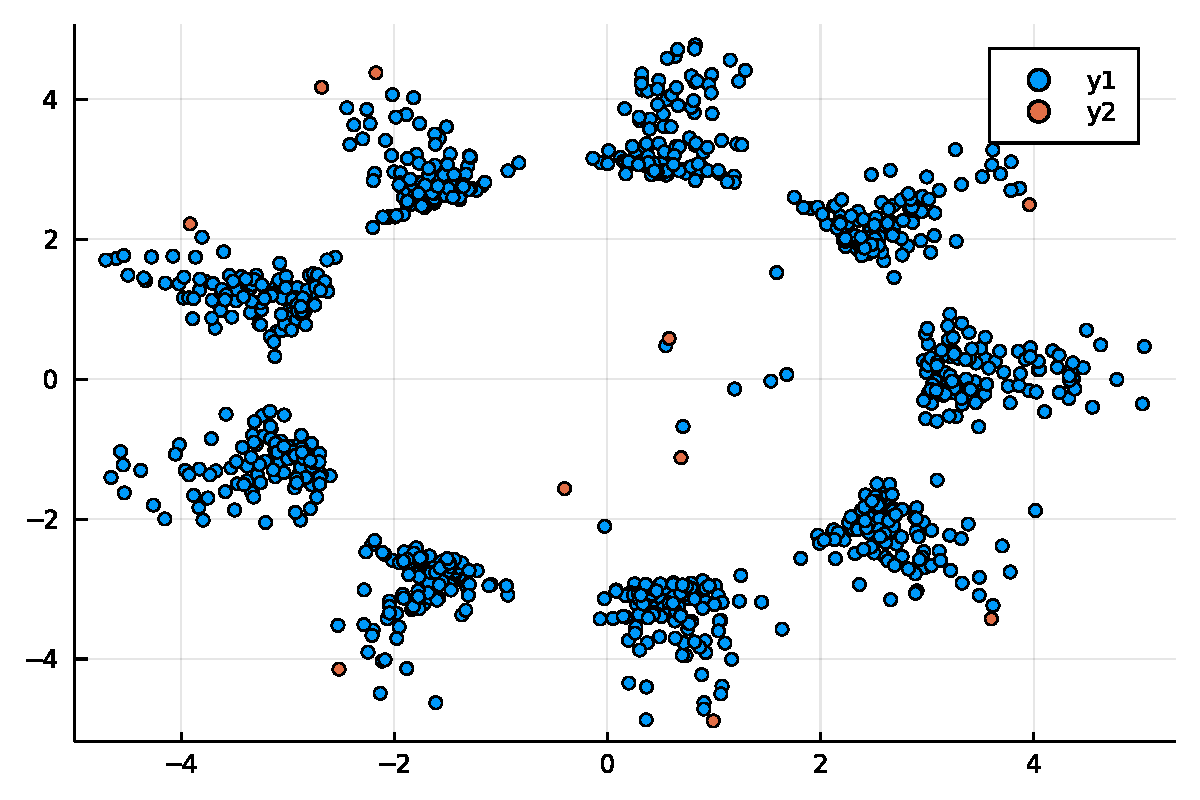
\includegraphics[width=\linewidth]{jl_uOl600/test1_6_1.pdf}

\section{Anomaly detection with quantile loss}
Model init. + train/anomaly data + training


\begin{lstlisting}
(*@\HLJLn{m}@*) (*@\HLJLoB{=}@*) (*@\HLJLnf{sptn}@*)(*@\HLJLp{(}@*)(*@\HLJLni{2}@*)(*@\HLJLp{,}@*) (*@\HLJLni{9}@*)(*@\HLJLp{,}@*) (*@\HLJLni{1}@*)(*@\HLJLp{)}@*)

(*@\HLJLn{x{\_}n}@*) (*@\HLJLoB{=}@*) (*@\HLJLnf{flower2}@*)(*@\HLJLp{(}@*)(*@\HLJLni{1000}@*)(*@\HLJLp{,}@*) (*@\HLJLn{npetals}@*)(*@\HLJLoB{=}@*)(*@\HLJLni{9}@*)(*@\HLJLp{)}@*)
(*@\HLJLn{x{\_}a}@*) (*@\HLJLoB{=}@*) (*@\HLJLnf{randn}@*)(*@\HLJLp{(}@*)(*@\HLJLni{2}@*)(*@\HLJLp{,}@*) (*@\HLJLni{10}@*)(*@\HLJLp{)}@*)
(*@\HLJLnf{scatter}@*)(*@\HLJLp{(}@*)(*@\HLJLn{x{\_}n}@*)(*@\HLJLp{[}@*)(*@\HLJLni{1}@*)(*@\HLJLp{,}@*) (*@\HLJLoB{:}@*)(*@\HLJLp{],}@*) (*@\HLJLn{x{\_}n}@*)(*@\HLJLp{[}@*)(*@\HLJLni{2}@*)(*@\HLJLp{,}@*) (*@\HLJLoB{:}@*)(*@\HLJLp{])}@*)
(*@\HLJLnf{scatter!}@*)(*@\HLJLp{(}@*)(*@\HLJLn{x{\_}a}@*)(*@\HLJLp{[}@*)(*@\HLJLni{1}@*)(*@\HLJLp{,}@*) (*@\HLJLoB{:}@*)(*@\HLJLp{],}@*) (*@\HLJLn{x{\_}a}@*)(*@\HLJLp{[}@*)(*@\HLJLni{2}@*)(*@\HLJLp{,}@*) (*@\HLJLoB{:}@*)(*@\HLJLp{])}@*)
(*@\HLJLn{x}@*) (*@\HLJLoB{=}@*) (*@\HLJLnf{shuffleobs}@*)(*@\HLJLp{(}@*)(*@\HLJLnf{hcat}@*)(*@\HLJLp{(}@*)(*@\HLJLn{x{\_}n}@*)(*@\HLJLp{,}@*) (*@\HLJLn{x{\_}a}@*)(*@\HLJLp{))}@*)
(*@\HLJLcs{{\#}scatter(x[1,}@*) (*@\HLJLcs{:],}@*) (*@\HLJLcs{x[2,}@*) (*@\HLJLcs{:])}@*)
(*@\HLJLn{{\_}data}@*) (*@\HLJLoB{=}@*) (*@\HLJLn{Iterators}@*)(*@\HLJLoB{.}@*)(*@\HLJLnf{repeated}@*)(*@\HLJLp{((),}@*) (*@\HLJLni{100}@*)(*@\HLJLp{)}@*)

(*@\HLJLnf{loss}@*)(*@\HLJLp{()}@*) (*@\HLJLoB{=}@*) (*@\HLJLoB{-}@*)(*@\HLJLnf{quantile{\_}loss}@*)(*@\HLJLp{(}@*)(*@\HLJLn{m}@*)(*@\HLJLp{,}@*) (*@\HLJLn{x}@*)(*@\HLJLp{,}@*) (*@\HLJLnfB{0.01}@*)(*@\HLJLp{,}@*) (*@\HLJLn{range}@*)(*@\HLJLoB{=}@*)(*@\HLJLp{(}@*)(*@\HLJLni{0}@*)(*@\HLJLp{,}@*) (*@\HLJLni{40}@*)(*@\HLJLp{))}@*)

(*@\HLJLn{ps}@*) (*@\HLJLoB{=}@*) (*@\HLJLn{Flux}@*)(*@\HLJLoB{.}@*)(*@\HLJLnf{params}@*)(*@\HLJLp{(}@*)(*@\HLJLn{m}@*)(*@\HLJLp{)}@*)

(*@\HLJLn{opt}@*) (*@\HLJLoB{=}@*) (*@\HLJLnf{ADAM}@*)(*@\HLJLp{(}@*)(*@\HLJLnfB{0.1}@*)(*@\HLJLp{)}@*)
(*@\HLJLn{Flux}@*)(*@\HLJLoB{.}@*)(*@\HLJLn{Optimise}@*)(*@\HLJLoB{.}@*)(*@\HLJLnf{train!}@*)(*@\HLJLp{(()}@*) (*@\HLJLoB{->}@*) (*@\HLJLnf{loss}@*)(*@\HLJLp{(),}@*) (*@\HLJLn{ps}@*)(*@\HLJLp{,}@*) (*@\HLJLn{{\_}data}@*)(*@\HLJLp{,}@*) (*@\HLJLn{opt}@*)(*@\HLJLp{)}@*)
\end{lstlisting}


Heatmap of trained distribution


\begin{lstlisting}
(*@\HLJLn{xx}@*) (*@\HLJLoB{=}@*) (*@\HLJLnf{reduce}@*)(*@\HLJLp{(}@*)(*@\HLJLn{hcat}@*)(*@\HLJLp{,[[}@*)(*@\HLJLn{v}@*)(*@\HLJLp{[}@*)(*@\HLJLni{1}@*)(*@\HLJLp{],}@*)(*@\HLJLn{v}@*)(*@\HLJLp{[}@*)(*@\HLJLni{2}@*)(*@\HLJLp{]]}@*) (*@\HLJLk{for}@*) (*@\HLJLn{v}@*) (*@\HLJLkp{in}@*) (*@\HLJLn{Iterators}@*)(*@\HLJLoB{.}@*)(*@\HLJLnf{product}@*)(*@\HLJLp{(}@*)(*@\HLJLoB{-}@*)(*@\HLJLnfB{10.0}@*)(*@\HLJLoB{:}@*)(*@\HLJLnfB{0.1}@*)(*@\HLJLoB{:}@*)(*@\HLJLni{10}@*)(*@\HLJLp{,}@*) (*@\HLJLoB{-}@*)(*@\HLJLnfB{10.0}@*)(*@\HLJLoB{:}@*)(*@\HLJLnfB{0.1}@*)(*@\HLJLoB{:}@*)(*@\HLJLni{10}@*)(*@\HLJLp{)])}@*)
(*@\HLJLn{res}@*) (*@\HLJLoB{=}@*) (*@\HLJLnf{reshape}@*)(*@\HLJLp{(}@*)(*@\HLJLnf{logpdf}@*)(*@\HLJLp{(}@*)(*@\HLJLn{m}@*)(*@\HLJLp{,}@*) (*@\HLJLn{xx}@*)(*@\HLJLp{),}@*) (*@\HLJLni{201}@*)(*@\HLJLp{,}@*) (*@\HLJLni{201}@*)(*@\HLJLp{)}@*)
(*@\HLJLn{Plots}@*)(*@\HLJLoB{.}@*)(*@\HLJLnf{heatmap}@*)(*@\HLJLp{(}@*)(*@\HLJLn{exp}@*)(*@\HLJLoB{.}@*)(*@\HLJLp{(}@*)(*@\HLJLn{res}@*)(*@\HLJLp{))}@*)
\end{lstlisting}

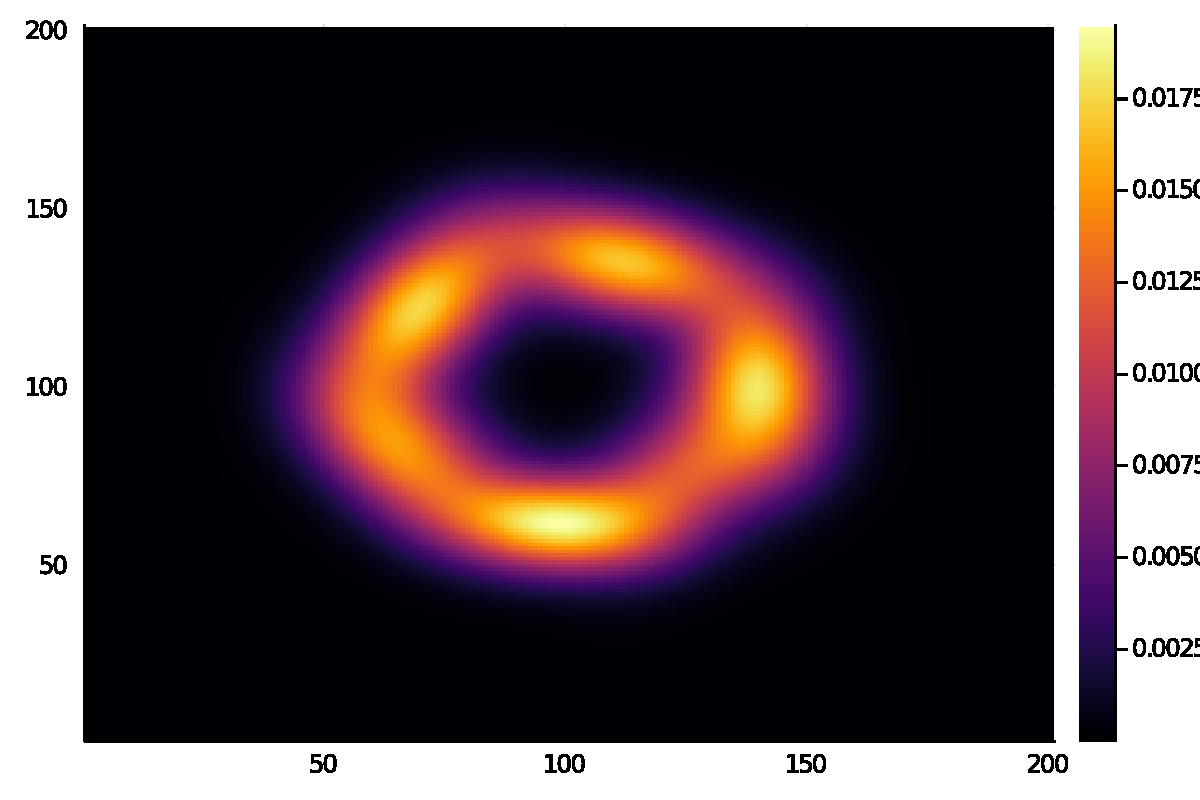
\includegraphics[width=\linewidth]{jl_uOl600/test1_8_1.pdf}

Scatter plot of anomaly detection.


\begin{lstlisting}
(*@\HLJLn{lkl}@*) (*@\HLJLoB{=}@*) (*@\HLJLnf{logpdf}@*)(*@\HLJLp{(}@*)(*@\HLJLn{m}@*)(*@\HLJLp{,}@*) (*@\HLJLn{x}@*)(*@\HLJLp{)}@*)
(*@\HLJLn{\ensuremath{\theta}}@*) (*@\HLJLoB{=}@*) (*@\HLJLnf{quantile{\_}tresh}@*)(*@\HLJLp{(}@*)(*@\HLJLn{lkl}@*)(*@\HLJLp{,}@*) (*@\HLJLnfB{0.01}@*)(*@\HLJLp{)}@*)

(*@\HLJLn{anom}@*)(*@\HLJLp{,}@*) (*@\HLJLn{norms}@*) (*@\HLJLoB{=}@*) (*@\HLJLnf{tresh{\_}lkl}@*)(*@\HLJLp{(}@*)(*@\HLJLn{m}@*)(*@\HLJLp{,}@*) (*@\HLJLn{x}@*)(*@\HLJLp{,}@*) (*@\HLJLn{\ensuremath{\theta}}@*)(*@\HLJLp{)}@*)
(*@\HLJLnf{scatter}@*)(*@\HLJLp{(}@*)(*@\HLJLn{norms}@*)(*@\HLJLp{[}@*)(*@\HLJLni{1}@*)(*@\HLJLp{,}@*) (*@\HLJLoB{:}@*)(*@\HLJLp{],}@*) (*@\HLJLn{norms}@*)(*@\HLJLp{[}@*)(*@\HLJLni{2}@*)(*@\HLJLp{,}@*) (*@\HLJLoB{:}@*)(*@\HLJLp{])}@*)
(*@\HLJLnf{scatter!}@*)(*@\HLJLp{(}@*)(*@\HLJLn{anom}@*)(*@\HLJLp{[}@*)(*@\HLJLni{1}@*)(*@\HLJLp{,}@*) (*@\HLJLoB{:}@*)(*@\HLJLp{],}@*) (*@\HLJLn{anom}@*)(*@\HLJLp{[}@*)(*@\HLJLni{2}@*)(*@\HLJLp{,}@*) (*@\HLJLoB{:}@*)(*@\HLJLp{])}@*)
\end{lstlisting}

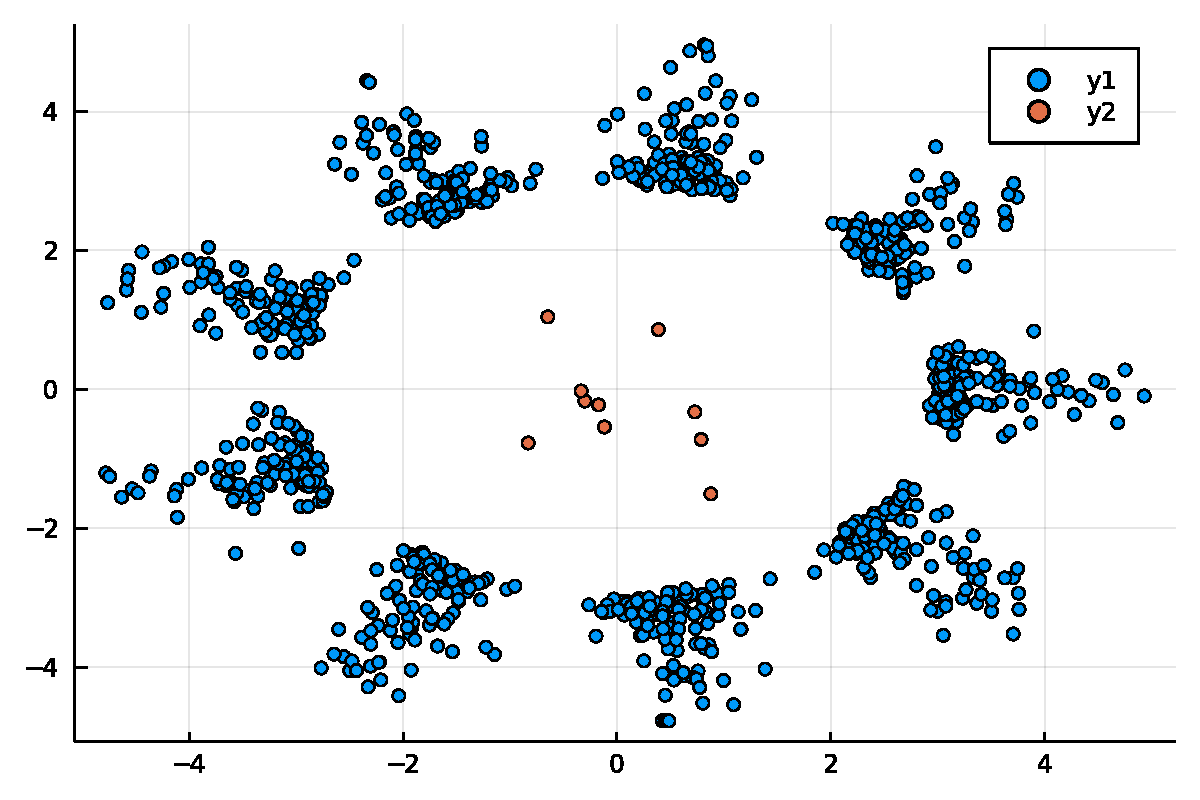
\includegraphics[width=\linewidth]{jl_uOl600/test1_9_1.pdf}


\end{document}
